\section{Ecossistema de software}

COMENTARIO GERAL: FALTAM REFERENCIAS BIBLIOGRAFICAS (USAR CITE SEM PARCIMONIA).


% ecossistema pode estar organizado em relacões de benefício mútuo

Ecossistema de software é definido, segundo \citeonline{manikas2013software},
como a interação entre diversos atores numa plataforma tecnológica comum
resultando em novas soluções de software ou novos serviços. 
Atores do ecossistema, motivados por um conjunto de interesses, conectam-se entre si e ao
próprio sistema numa relação simbiótica, fazendo a plataforma tecnológica
evoluir enquanto permite o envolvimento e contribuição de novos e diferentes
atores.

Nesta relação, os atores são beneficiados de formas diferentes a depender da
natureza do ecossistema. Num ambiente comercial, por exemplo, os atores são
beneficiados diretamente através de receita financeira (salário, prêmios, etc),
enquanto num sistema não-comercial os atores estão motivados por questões
não-monetárias, como fama, reconhecimento, ideologia, etc.

De modo geral, em ecossistemas de software, os benefícios recebidos pelos
atores e proporcionados pelo ecossistema, aumentam com o passar do tempo
por meio de uma relação de benefício mútuo. 
Este modelo geral de funcionamento, no entanto, pode variar 
a depender do contexto em que se insere o ecossistema.

%, o ecossistema de software acadêmico por
%exemplo possui a particularidade de estar inserido no sistema de reputação
%científica de alguma forma.

%os atores recebem mais (ou melhores) benefícios com o crescimento
%do ecossistema, o ecossistema oferece cada vez mais (ou melhores) benefícios
%com as atividades dos seus atores, resultando numa relação de benefício
%mútuo.

\section{Ecossistema de software acadêmico}

O ecossistema de software acadêmico possui a particularidade de se relacionar
com o sistema econômico de reputação científica, especialmente com o seu modelo
de publicações, influenciando e sendo influenciado diretamente pelo impacto de
suas publicações.

%e pelo seu sistema de crédito acadêmico.

% (5) Tools in mining software repositories \cite{chaturvedi2013tools}
% Faz uma revisão dos papers submetidos ao MSR desde 2007 até 2013 (?) e
% identifica data sets, ferramentas e técnicas utilizadas pelos autores, mais
% da metade dos papers usam ou criam ferramentas, categoriza as ferramentas em
% ferramentas novas, ferramentas tradicionais, protótipos e scripts para
% mineração de dados

Neste cenário, interessado em compreender as relações neste ecossistema,
\citeonline{howison2015understanding} criou um framework para pensar e refletir
sobre o processo de produção de software no meio científico, e identificou quatro
papéis básicos envolvidos no ecossistema de software acadêmico: 
(1) cientistas usuários finais, (2) produtores e distribuidores de software, (3)
administradores de infraestrutura e (4) pesquisadores preocupados com o
funcionamento do ecossistema como um todo.

\subsection{Cientistas usuários finais}

Cientistas ocupam papel chave no ecossistema de software acadêmico.
Em seus processos de investigação e experimentação, fazem uso crescente 
de software para coleta, gerenciamento, transformação, análise, modelagem e
visualização de dados. 
Além da preocupação com qualidade e usabilidade,
estes cientistas estão também preocupados com a disponibilidade e com a
capacidade do software em continuar sendo útil.

Finalmente, cientistas estão interessados também em saber o que outros 
cientistas estão usando em suas pesquisas. A alta adoção de um software, 
além de ser um bom indicador de qualidade, mantém os cientistas mais livres 
e com maior foco em suas próprias pesquisas, uma vez que podem encontrar
ajuda entre os seus pares para resolver questões sobre o uso do software.

%e de podendo ser utilizado em conjunto com outras
%soluções de software.

%garantir que o grupo de pesquisa, estudantes e colaboradores consigam 
% simplifica também o trabalho dos
%revisores pois encontrarão as mesmas facilidades no uso.

\subsection{Produtor e distribuidor de software acadêmico}

O papel de produtor e distribuidor de software costuma ser desempenhado por
equipes colaborando entre sí, geralmente compostas por cientistas 
da computação e cientistas do domínio onde a pesquisa se insere. Geralmente, 
o cientista da computação é o responsável por implementar os algoritmos, 
métodos ou resultados gerados pelo estudo.

Um desafio comum enfrentado neste papel é conseguir abstrair os problemas e
implementar soluções abrangentes em software. Muitas vezes, o software criado
fica confinado em seu laboratório ou grupo, mas eventualmente é compartilhado e
%potencialmente 
amplamente adotado, tornando o cientista autor do software e da
pesquisa parte do ecossistema \cite{howison2015understanding}.

%que podem ser adotadas por outros cientistas,
%especialmente em outros domínios. 

Entre as inúmeras preocupações do produtor e distribuidor de software, 
podemos destacar a preocupação acerca de como o software contribui para 
as investigações científicas que outros pesquisadores
estão realizando.
Alguns projetos são gerenciados no estilo de código aberto, e
têm atraído com sucesso contribuições de muitos cientistas, incluindo 
contribuidores que tem fazem pequenas, porém  substanciais contribuições.

%preocupam-se com o impacto cientifico tanto em termos de numero
%quando de tipos de usuários que seu software atinge, 

\subsection{Provedor de infraestrutura}

O provedor de infraestrutura é aquele que provê cojuntos de software aos
cientistas usuários finais. Este conjunto pode estar disponível em forma de
download para que seja utilizado em computadores pessoais ou pode estar
disponível em forma de serviços, como por exemplo, ciberinfraestrutura de
software.
%ciberinfraestrutura de software hospedados em centros de supercomputação
%usando provedores de computação em nuvem.

Do ponto de vista do ecossistema, os dois tipos de distribuição implicam nas
mesmas preocupações e questões: quem usa o software, qual versão é utilizada, 
qual a frequencia de atualização, entre outras.
% preocupações relacionadas à distribuição e uso.

\subsection{Pesquisador}

Este último papel, chamado de pesquisador num sentido amplo, refere-se a
qualquer pessoa preocupada com o funcionamento do ecossistema e com a sua
contribuição para a Ciência. O papel de pesquisador costuma ser desempenhado 
por agências de fomento ou por cientistas preocupados com o seu trabalho 
individual e com o impacto em seu campo de pesquisa.

As preocupações incluem questões sobre a operação do ecossistema
como um sistema que consome recursos (tempo, dinheiro e atenção) e afeta a
conduta da Ciência, tanto no geral como em campos específicos, 
e sobre a compreensão do comportamento desse sistema e de 
como pode ser influenciado.

\section{Modelo de desenvolvimento de software acadêmico}

% recurso, uso e impacto

Cada ator desempenha um papel importante na estabilidade e sustentabilidade do
ecossistema. Assim como nos ecossistemas naturais, o ecossistema de software
necessita de fornecimento constante de energia, seja na forma de
novos desenvolvimentos ou na forma de ações de manutenção \cite{dhungana2010software}.

Os atores participam dentro de seus próprios interesses, mas sempre causando
impacto no sistema como um todo. Cientistas usuários finais usam software
acadêmico (direta ou indiretamente) para fazer Ciência, resultando em impacto
científico. Tal impacto científico justifica novos investimentos, fazendo o
ecossistema crescer.

%a partir da evolução deste software ou a partir da produção de novo software.

\begin{figure}[h]
  \center
  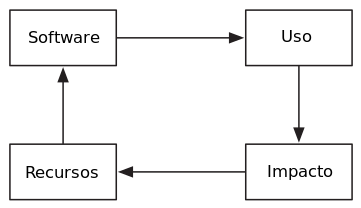
\includegraphics[scale=0.5]{imagens/process-model-scientific-software-dia.png}
  \caption{Um modelo de process de software na Ciência~\cite{howison2015understanding}}
  \label{process-model-scientific-software}
\end{figure}

A Figura \ref{process-model-scientific-software} apresenta um modelo de 
desenvolvimento de software acadêmico, explicitando as relações entre os elementos 
\textit{software}, \textit{recursos}, \textit{uso} e \textit{impactos}, detalhados a seguir.

\subsection{Software}

Software acadêmico ({\it academic software}) é todo software usado para
coletar, processar ou analisar resultados de pesquisas com intenção de
publicação na literatura acadêmica (periódicos, revistas, conferências,
monografias, livros ou teses), incluindo desde protótipos escritos pelos próprios
cientistas, a produtos completos desenvolvidos profissionalmente
\cite{allen2017engineering}.

%Podem ser encontrados na literatura acadêmica com outros nomes,
%{\it research tool} \cite{Portillo12},
%{\it research-originated software} \cite{Kon2011},
%{\it research software} \cite{hettrick_2014_14809} ou
%{\it scientific software} \cite{segal2008developing},
%esses artefatos tem sido estudados dos mais variados pontos
%de vista, desde de sua qualidade interna, até o impacto que
%causam no meio científico.

Entre as inúmeras funções desempenhadas pelo software acadêmico em suas
pesquisas, identificam-se motivações distintas para a criação, 
usadas para agrupar ou categorizar cada software [CITAR]:

\begin{enumerate}
  \item Ganho monetário direto (software comercial, desenvolvedores de software contratados);
  \item Reputação acadêmica (software incidental, dirigido pela necessidade científica direta);
  \item Prática de software paralela (scientific needed enhanced by publishing 'software papers' 
alongside domain research);  [NAO ENTENDI]
  \item Software de uma subárea de pesquisa (reputação direta pelo trabalho do software);
  \item Híbridos como licença-dual e 'software work' dentro de grandes colaborações (software como uma contribuição científica direta).
\end{enumerate}


EXPLICAR MELHOR CATEGORIAS ACIMA;FIQUEI CONFUSA.

\subsection{Recursos}

Os recursos investidos na produção de software acadêmico vêm de diversas fontes,
incluindo ganhos monetários diretos, recursos alocados em projetos, e colaboração
entre laboratórios de pesquisa. Grande parte dos recursos vem do ``tempo livre'' 
dos pesquisadores em busca de soluções para suas pesquisas e 
perpassa por financiamentos diversos, carreira individual do cientista,
estudantes de graduação, prêmios, etc.

Independente da origem do recurso, grande parte do desenvolvimento de software 
acadêmico é realizado pelos próprios cientistas.
Esta tendência tem sido interpretada como um reflexo do conhecimento sobre
domínio da pesquisa muitas vezes necessário ao desenvolvedor deste software
\cite{segal2008developing, hettrick_2014_14809, momcheva2015software}.

\subsection{Uso}

% ... software é distribuido, utilizado e dá suporte à ciencia, gerando impacto ...

Metade dos pesquisadores de todas as áreas da Ciência fazem uso
intenso de software acadêmico, desde grupos trabalhando exclusivamente com
problemas computacionais até grupos em laboratórios tradicionais ou em campo
\cite{wilson2014best}.

Este uso é mencionado em suas pesquisas, por meio de citação formal ou
informal. Estas menções são parte do sistema econômico de reputação científica
e causam impacto científico direto tanto na publicação quanto no ecossistema de
software acadêmico.

Este impacto direto geralmente justifica o investimentos de novos recursos no
ecossistema, seja para fins de planejamento, como retrospectiva para avaliar
investimentos já realizados ou para promover evolução do software acadêmico.

\subsection{Impacto científico}

% ... impacto científico justifica e potencialmente gera mais recurso ...
% \cite{katz2014transitive}

Ao longo da história, a citação formal tem sido utilizada para garantir
autenticidade e autoridade, ao invés de crédito e reconhecimento.
Na história ocidental, a citação surge no final do século XVI e, 
no início do século XVIII surgem o sistema legal por trás do sistema de citações 
e a lei de ``copyright'' para garantir os direitos dos autores.

Apesar do grande uso para garantir autenticidade e autoridade, o sistema de
citações e a informação sobre a autoria das publicações tem sido realmente
utilizado para avaliações importantes dentro do corpo científico.
Por exemplo, ``backward citing'' tem sido utilizado para se certificar quem de fato
contribuiiu para um certo avanço ou descoberta, e ``forward citing''
tem sido usada em casos onde se quer entender como uma idéia foi usada após o
seu surgimento ou publicação.

%Tradicionalmente, um autor cita um artigo anterior adicionando uma referência 
%ao autor, título, local de publicação, etc.

Conhecimento novo é claramente construído a partir do conhecimento passado e o
sistema de citações formais tem promovido avanços significativos.
No entanto, esse conceito não tem funcionado tão bem para produtos digitais como o
software, que muitas vezes depende de outro software, fragmentos de código, e
algoritmos.

Este debate ocorre há bastante tempo entre as diversas áreas da
bibliometria, cienciometria, altmetria e áreas similares.
Por exemplo, o fator de impacto, proposto em 1955 [CITAR],
apesar de contribuir para a Ciência, por vezes é utilizado da forma errada 
e mostra as deficiências de lidar bem com produtos digitais gerados durante pesquisas.

%%% PAREI AQUI %%%

\section{Sustentabilidade do ecossistema de software acadêmico}

% problemas identificados no ecossistema de software acadêmico

%Um estudo sobre ecossistema de software acadêmico percebeu através dos relatos
%de grande parte dos colaboradores participantes do estudo que os projetos de software
%acadêmicos desenvolvidos na própria academia 

O ecossistema de software acadêmico sofre de {\it ``dysfunctional chaotic
churn''}:

\begin{quote}
Existência de muitos projetos, com poucos usuários, com
ciclos de vida curtos, que terminam em paralelo ao financiamento inicial,
comunidades desconectadas e paralelas, incompatibilidades entre projetos, e
tentativas aparentemente não coordenadas de ``reiniciar'' tudo ({\it re-boots})
\cite{howison2015understanding}.
\end{quote}

Este problema apesar de ser apenas uma percepção coincide com inúmeras
evidências a respeito de problemas com o desenvolvimento, reconhecimento e
sustentabilidade do software acadêmico \cite{allen2017engineering}.

%sabe-se que parte dos problemas são realmente fato, por exemplo,
%o {\it Dagstuhl Perspective Workshop}, evento organizado por um grupo de
%pesquisadores sêniores de renome internacional, realizado anualmente na
%universidade de Dagstuhl\footnote{\url{http://www.dagstuhl.de}} com o objetivo
%refletir sobre o estado da ciência da computação explorando tópicos novos e
%emergentes, em sua mais recente edição o workshop debateu sobre software

\subsection{Desenvolvimento}

O desenvolvimento de software acadêmico exige, muitas vezes, conhecimento
específico sobre o domínio do estudo sendo realizado,
por exemplo, entender como o DNA genômico
se transforma em cristais de proteína, ou estar familiarizado com os meandros
da dinâmica dos fluidos, ou saber como resolver 20 equações diferenciais
parciais simultâneas \cite{segal2008developing}.

Isto explica a grande participação dos cientistas no desenvolvimento de
software acadêmico, estudos tem mostrado que no reino unido entre todas as
áreas da ciência 56\% dos cientistas estão envolvidos no desenvolvimento de
software acadêmico, outros estudos em grupos específicos mostram números ainda
maiores, na astronomia, por exemplo, 90\% dos cientistas desenvolvem software
acadêmico \cite{hettrick_2014_14809, momcheva2015software}.

No entanto, a maior parte dos cientistas nunca tiveram treinamento algum sobre como escrever
softwares de forma eficiente, muitos não testam ou documentam os seus
softwares, faltam práticas básicas de desenvolvimento, como escrever código
legível, revisão de código, controle de versão, testes unitários, entre outros
\cite{wilson2017good}.

Isto tem ocasionado sérios erros computacionais em conclusões centrais da
literatura acadêmica, gerando retrabalho para retratar tais erros nas mais
diversas áreas da ciência \cite{Merali2010Computational}. Dados são perdidos,
análises levam mais tempo que o necessário e os pesquisadores não conseguem a
eficiência que poderiam ter ao trabalhar com softwares acadêmicos
\cite{wilson2017good}.  Causando um impacto negativo na visibilidade dos
softwares acadêmicos \cite{howison2013, katz2014transitive} e na capacidade de
serem encontrados e compartilhados.

\subsection{Reconhecimento}

% visibilidade

Apesar do crescimento no uso de software e na consequente dependência entre
cientistas de todos os campos, tornando o software acadêmico parte integral da
prática científica, apesar do apelo da comunidade científica para que o
software acadêmico seja tratado como cidadão de primeira classe, estudos tem
mostrado que muitas pesquisas não mencionam sequer o uso de software acadêmico
em suas publicações mesmo tendo feito uso de tais artefatos
\cite{momcheva2015software} \cite{howison2016software}.

Isto tem prejudicado a visibilidade do software acadêmico causando impacto
negativo em seu ecossistema, um software invisível é frequentemente excluído de
revisões por pares, uma atividade que costuma contribuir para a qualidade geral
do trabalho publicado, além disso, o
impacto negativo na visibilidade do software acadêmico faz surgir uma
série de questionamentos sobre a sua qualidade e também sobre a
capacidade de ser encontrado, compartilhado e co-desenvolvido
\cite{howison2013, katz2014transitive} \cite{howison2016software}.

Apesar de nem sempre ser possível, ou viável, ter tudo dentro de padrões
estritos, é preciso estar consciente das boas práticas ao produzir e utilizar
softwares acadêmicos, tanto para melhorar a própria abordagem quanto para
revisar outros trabalhos \cite{wilson2014best}. Um software acadêmico em bom
funcionamento devem atingir não apenas os objetivos de entendimento e
transparencia, mas também os objetivos voltados para replicação
\cite{Stodden2010}, seja logo após sua publicação, seja daqui a 10 ou 50 anos.

\subsection{Sustentabilidade}

O desenvolvimento de software sustentável tem sido identificado como um desafio
chave no campo da ciência e da engenharia computacional, se sustentabilidade
não for levada em consideração em projetos de software, não importa qual o
domínio ou qual o propósito do software, perde-se a oportunidade de causar
mudanças positivas no planeta e na sociedade.

Sustentabilidade apesar de ser um conceito complexo e com mútiplas dimensões,
levando a debates profundos, possui um conceito geral bastante simples, refe-se à
capacidade de perdurar e de continuar sendo suportado ao longo do tempo, isto
implica na qualidade de longevidade e manunetabilidade do software
\cite{venters2014software}.

Software sustentável é aquele que continua a estar disponível no futuro, em
novas plataformas, atendendo continuamente às novas necessidades do ambiente
através de uma adequada evolução frente as condições em constante mudança
\cite{allen2017engineering}.

No entando, estudos mostram o decaimento de URLs ao longo do tempo, em
publicações com produção de artefatos digitais disponibilizados nestes
endereços tem uma tendência a tornarem-se indisponíveis ao longo dos anos
\cite{wren2017use}.

Isto tem motivado iniciativas de tornar estes artefatos duráveis e disponíveis,
visando especialmente garantir a longevidade dos artefatos e proporcionar que
um segundo pesquisador receba todos os benefícios do trabalho duro do primeiro
pesquisador \cite{king1995replication},
o {\it Journal of the American Statistical Association (JASA)}, por
exemplo, tem insistido na necessiade de estar disponíveis código e dados ao
menos durante a revisão dos manuscritos \cite{baker2016scientists}, agências de
financiamento, como o {\it US National Science Foundation}, estão começando a
reconhecer produtos de pesquisa, como software, assim como fazem com as
publicações, tornando o software produzido em pesquisas cidadão de primeira
classe na ciência.

%Iniciativas desta natureza resolvem o problema de disponibilidade destes
%artefatos mas ainda não garantem adequada evolução frente a contínua mudança
%do ambiente, apesar de sustentabilidade não implicar diretamente em qualidade,
%
%Tanto a ciência quanto a
%engenharia dependem de resultados incrementais para sua evolução. No terceiro
%compromisso, relacionado ao conceito {\it desenvolvimento}, o Dagstuhl
%Manifesto enfatiza a necessidade de medir a qualidade e a sustentabilidade dos
%softwares científicos, tanto a priori quanto a posteriori.

Isto garante longevidade mas não implica em boa manutenabilidade, a qualidade
dos softwares acadêmicos tem sido questionada, a maioria dos cientistas autores
de software não sabe o quão confiável seu software é
\cite{Merali2010Computational}, muitos dos projetos de software acadêmico estão
em estado inicial de desenvolvimento \cite{marshall2013tools}, poucos foram
testados fora do contexto onde foram desenvolvidos \cite{Portillo12}.

\subsubsection{Manutenabilidade}

% falar de manutenabilidade como um eixo dentro de sustentabilidade técnica

Manutenabilidade é uma característica de qualidade que indica o quão fácil é
realizar atividades de evolução e manutenção em software, um aspecto
importante aos pesquisadores interessados em adaptar software acadêmico, algo
muitas vezes necessário ao reproduzir pesquisas anteriores \cite{Peng2011}.

Manutenabilidade é uma característica de qualidade externa que indica o quão
fácil é realizar atividades de evolução e manutenção em componentes de
software, ela pode ser medida através de características de qualidade interna,
uma vez que grande parte dos engenheiros de software assumem que uma boa
estrutura interna resulta em boa qualidade externa \cite{Fenton2014}. A
estrutura interna de um software pode ser avaliada através da sua complexidade,
uma característica bastante referenciada na literatura como um importante
indicador de qualidade, estudos mostram que quanto maior a complexidade, maior
é o esforço de manutenção \cite{hashim1996software, Darcy2005}, em especial a
complexidade estrutural, uma medida definida em termos de acoplamento e coesão
\cite{Terceiro2012}.

A adoção e uso de software acadêmico está relacionado
também à sua qualidade, portanto é impoprtante medir e coletar sua qualidade de
alguma forma, qualidade é um vasto assunto, um dos problemas comuns enfrentado
pelos pesquisadores que desenvolvem tais softwares é a manutenabilidade
\cite{Prlic2012}.

Estudos tem mostrado que grande parte das ferramentas de software criadas na
academia estão em estado inicial de desenvolvimento \cite{marshall2013tools} e
que apenas uma pequena porcentagem são testados fora do contexto onde foi
desenvolvido \cite{Portillo12}.

%%%%%%%%%%%%%%%%%%%%%%%%%%%%%%%%%%%%%%%%%%%%%%%%%%%%%%%%%%%%%%%%%%%%%

%Cita um mapeamento feito sobre estudos que criam ferramentas para apoio a
%revisão sistemática no domínio de SE, 14 estudos foram selecionados, ao final
%apenas 8 tinham proposta de ferramentas, ao final conclui que as ferramentas
%encontradas estão em estado inicial de desenvolvimento \cite{marshall2013tools}.

%Cita um mapeamento sistemático com objetivo de encontrar ferramentas de
%comunicação e coordenação para suporte a times altamente distribuidos
%gograficamente, encontrou 132 ferramentas, para uso em projetos de software
%global. A maioria destas ferramentas foram desenvolvidas em centros de
%pesquisas, e apenas uma pequena porcentagem (18.9\%) foram testados fora do
%seu contexto onde foi desenvolvido \cite{Portillo12}.

%Computer systems research spans sub-disciplines that in-
%clude embedded and real-time systems, compilers, network-
%ing, and operating systems. Our contention is that a number
%of structural factors inhibit quality research. We highlight
%some of the factors we have encountered in our work and ob-
%served in published papers and propose solutions that could
%both increase the productivity of researchers and the quality
%of their output \cite{Vitek2011}.

%Além da aplicação, estes softwares variam também no papel que ocupam em suas
%pesquisas, alguns fazem parte dos resultados da pesquisa, como por exemplo,
%propostas de novos algoritmos ou técnicas de produção, outros são utilizados
%como parte do método de pesquisa, como coleta ou análise de dados, sendo que
%estes papeis não são excludentes.
%
%estes costumam ser citados pelos seus autores como uma das contribuições do
%estudo, seja principal ou secundária, 
%Esses softwares podem, de fato, ser um software de simulação complexo desenvolvido
%e executado em um computador de alto desempenho, mas também pode ser um
%software desenvolvido em um PC para incorporação em instrumentos; para
%manipular, analisar ou visualizar dados; ou para orquestrar fluxos de trabalho.

%e à medida
%que percebe-se que os softwares estão se tornando parte integrante dos
%processos, ferramentas e produção científicas, torna-se necessário e urgente
%discutir o seu desenvolvimento, visibilidade, qualidade e sustentabilidade.

% mostrar os beneficios da ciencia aberta, ciberinfraestrutura, etc
% * (favorecendo a ciencia e tornando a vida mais feliz para todos)

% mostrar os problemas para a ciência como um todo
% * causando problemas para o progresso de ciência, dados perdidos, etc, retrabalho
%   dificuldade de reprodução, etc...

%, não apenas técnica, mas também a
%capacidade de ser encontrado, compartilhado e co-desenvolvido, qualidades
%importantes para a evolução do próprio software, mas também extremamente útil
%para um uso eficiente dos limitados recursos da ciência \cite{howison2013,
%katz2014transitive}.

%contradizendo as boas
%práticas de qualquer projeto experimental, de ter {\it laboratory
%notebooks}\footnote{\url{https://en.wikipedia.org/wiki/Lab_notebook}}, dados
%organizados, passos documentados, e projeto estruturado para reprodutibilidade.

%softwares acadêmicos, assim
%como qualquer outro aparato experimental, são tão importantes para a ciência
%quanto são os telescópios ou tubos de ensaio \cite{wilson2014best}.

%Cientistas gastam mais tempo hoje utilizando e desenvolvendo softwares do que
%gastavam no passado.

%Software is a critical part of modern research and yet there is little support across the
%scholarly ecosystem for its acknowledgement and citation. Inspired by the activities
%of the FORCE11 working group focused on data citation, this document
%summarizes the recommendations of the FORCE11 Software Citation Working
%Group and its activities between June 2015 and April 2016. Based on a review of
%existing community practices, the goal of the working group was to produce a
%consolidated set of citation principles that may encourage broad adoption of a
%consistent policy for software citation across disciplines and venues. Our work is
%presented here as a set of software citation principles, a discussion of the motivations
%for developing the principles, reviews of existing community practice, and a
%discussion of the requirements these principles would place upon different
%stakeholders. Working examples and possible technical solutions for how these
%principles can be implemented will be discussed in a separate paper.
%\cite{smith2016software}

%Improving academic software engineering projects: A comparative study of academic and industry projects
%(compara as praticas de desenvolvimento da industria e academia e sugere melhorias, 1998!)
%https://link.springer.com/article/10.1023%2FA%3A1018925902814?LI=true

% papel pesquisador no ecossistema de soft academico
%
%Essas preocupações gerais sugerem um conjunto de questões específicas, com foco
%em padrões globais e padrões emergentes dentro do ecossistema, incluindo: Quais
%recursos foram destinados à produção de software? Quantos usuários ou
%comunidades de usuários têm projetos? Quais são os impactos científicos desse
%uso? Os números de usuários crescem? Os projetos possuem recursos e habilidades
%suficientes para gerenciar seu crescimento? Quais projetos possuem
%funcionalidades sobrepostas? Há quanto tempo os pedaços de software e projetos
%persistem? Nós desconectamos as comunidades de usuários e desenvolvedores? São
%componentes específicos, ou camadas de componentes, faltam? Que código
%geralmente é usado em conjunto; são os projetos e as pessoas que produzem esses
%componentes se comunicando adequadamente? Como podemos sustentar o software
%crítico?
%
%Aqui há uma clara tensão entre um desejo de flexibilidade e liberdade, ligado
%às expectativas de inovação científica e desejos de estruturas de autoridade e
%controle de coordenação. As questões de influência incluem: como os programas
%de financiamento e quais os requisitos em suas chamadas, resultaram em software
%amplamente utilizado e impacto científico substancial? Quais são as
%características dos campos que alcançaram maior coalescência? Quais jornais e
%conferências têm políticas exemplares? Como o trabalho de software é visto
%dentro das práticas de contratação e avaliação, como os casos de posse?
%
%\cite{howison2015understanding}

%Ao longo da história, a citação formal foi para autenticação e autoridade, em
%vez de de crédito e reconhecimento ou atribuição. A  científico citação na
%história ocidental aparece no final dos anos 1500. No início dos anos 1700, a
%citação também aparece no sistema legal como método de compreensão dos
%precedentes \cite{katz2014transitive}.

%A ideia de direitos autorais como reconhecendo aos direitos dos seus autores
%também surge nesse tempo, 1710, talvez devido a uma lenta tendência social
%societária de reconhecer a propriedade intelectual, uma idéia que parece ter se
%desenvolvido ao lado da imprensa]. Observe que a autoria de papers é realmente
%usado para notar os autores reais do artigo quanto para notar os contribuidores
%do projeto.
%Para muitos desses, o
%identificador que deve ser citado - um "nome" que se refere a um produto único
%não é claro.

%Additionally, if a cited library depends
%on another library, the contribution of this second library
%is not captured. Citation of a dataset should perhaps give
%credit to the people who gathered the data, as well as
%those who curated it, but the paper author may not know
%or be able to find these details.

%Mas independente de como seja calculado o impacto científico de uma determinada
%pesquisa o impacto causado se reverte potencialmente em mais recursos que
%poderão ser reinvestidos no próprio ecossistema onde o software está inserido.

%Science Code Manifesto \cite{barnes2013science}.
%Foco em código fonte escrito especificamente para processar dados de
%publicações, afirma que ``todo código fonte escrito especificamente para
%processar dados de uma publicação deve estar disponível para os revisores e
%leitores do paper''.

%Sustentabilidade é um conceito guarda chuva composto de múltiplas dimensões, em
%sua dimensão técnica, chamada sustentabilidade técnica, temos a preocupação com
%a longevidade da informação, dos sistemas, e infraestrutura, e sua adequada
%evolução frente as condições do ambiente em constante mudança.

%citações formais facilitam e promovem o avanço
%da ciência, mesmo diante da falta de um padrão para citar artefatos digitais
%\cite{allen2014credit}.

%Um estudo recente com 90 artigos de diversas áreas da biologia, selecionados
%aleatoriamente entre publicações usando softwares como método, mostrou que
%apenas 59 mencionavam o uso de softwares de alguma forma, os demais 31 artigos,
%apesar de usar software acadêmico, não mencionavam nada a respeito
%\cite{howison2016software}, apenas entre 31\% e 43\% das menções aos softwares
%acadêmicos envolvem citação formal.

%Não existe ainda amadurecimento suficiente sobre como citar softwares e
%outros artefatos digitais em pesquisas científicas, não temos um padrão de como fazê-lo,
%cada autor cita à sua maneira, muitas vezes ao longo do texto, outras em seções
%específicas sobre a implementação do software, nem semprem informam onde
%encontrar uma cópia do software, ou ainda nem sobre o modelo em que o software
%é distribuído, ou se é de alguma forma distribuído ao público.

%Entre os softwares acadêmicos desenvolvidos por cientistas como apoio em suas
%pesquisas, não é raro que pesquisadores deixem de disponibilizar estes artefatos,
%assim como outros desdobramentos da pesquisa, como dados e outros. Ou ainda,
%mesmo disponibilizando tais artefatos em locais de público acesso, com o tempo,
%tais locais se tornam indisponíveis inviabilizando a obtenção de tais
%artefatos.

%A comunidade tem refletido sobre os problemas relacionados ao
%desenvolvimento, promoção e sustentabilidade desses softwares, e o
%impacto que tais problemas causam no meio científico \cite{allen2017engineering}.

%, e faz
%surgir questionamentos sobre sua qualidade, não apenas técnica, mas também a
%capacidade de ser encontrado, compartilhado e co-desenvolvido, qualidades
%importantes para a evolução do próprio software, mas também extremamente úteis
%para o uso eficiente dos limitados recursos da ciência \cite{howison2013,
%katz2014transitive}.
